%
% $RCSfile$
%
% Copyright (c) 2005-2006. Christian Heller. All rights reserved.
%
% Permission is granted to copy, distribute and/or modify this document
% under the terms of the GNU Free Documentation License, Version 1.1 or
% any later version published by the Free Software Foundation; with no
% Invariant Sections, with no Front-Cover Texts and with no Back-Cover
% Texts. A copy of the license is included in the section entitled
% "GNU Free Documentation License".
%
% http://www.cybop.net
% - Cybernetics Oriented Programming -
%
% http://www.resmedicinae.org
% - Information in Medicine -
%
% Version: $Revision$ $Date$ $Author$
% Authors: Christian Heller <christian.heller@tuxtax.de>
%

\subsubsection{Module Modelling}
\label{module_modelling_heading}

When CYBOI had become more stable (besides the extensions that were -- and are
-- frequently implemented, development could focus on the actual application
again. From now on, \emph{Res Medicinae} modules only had to be \emph{modelled}
in CYBOL, but no longer had to be \emph{coded} in a programming language. The
designed state- and logic knowledge, existing in form of CYBOL templates,
already represented the complete application; no further implementation phase
was needed.

\begin{figure}[ht]
    \begin{center}
        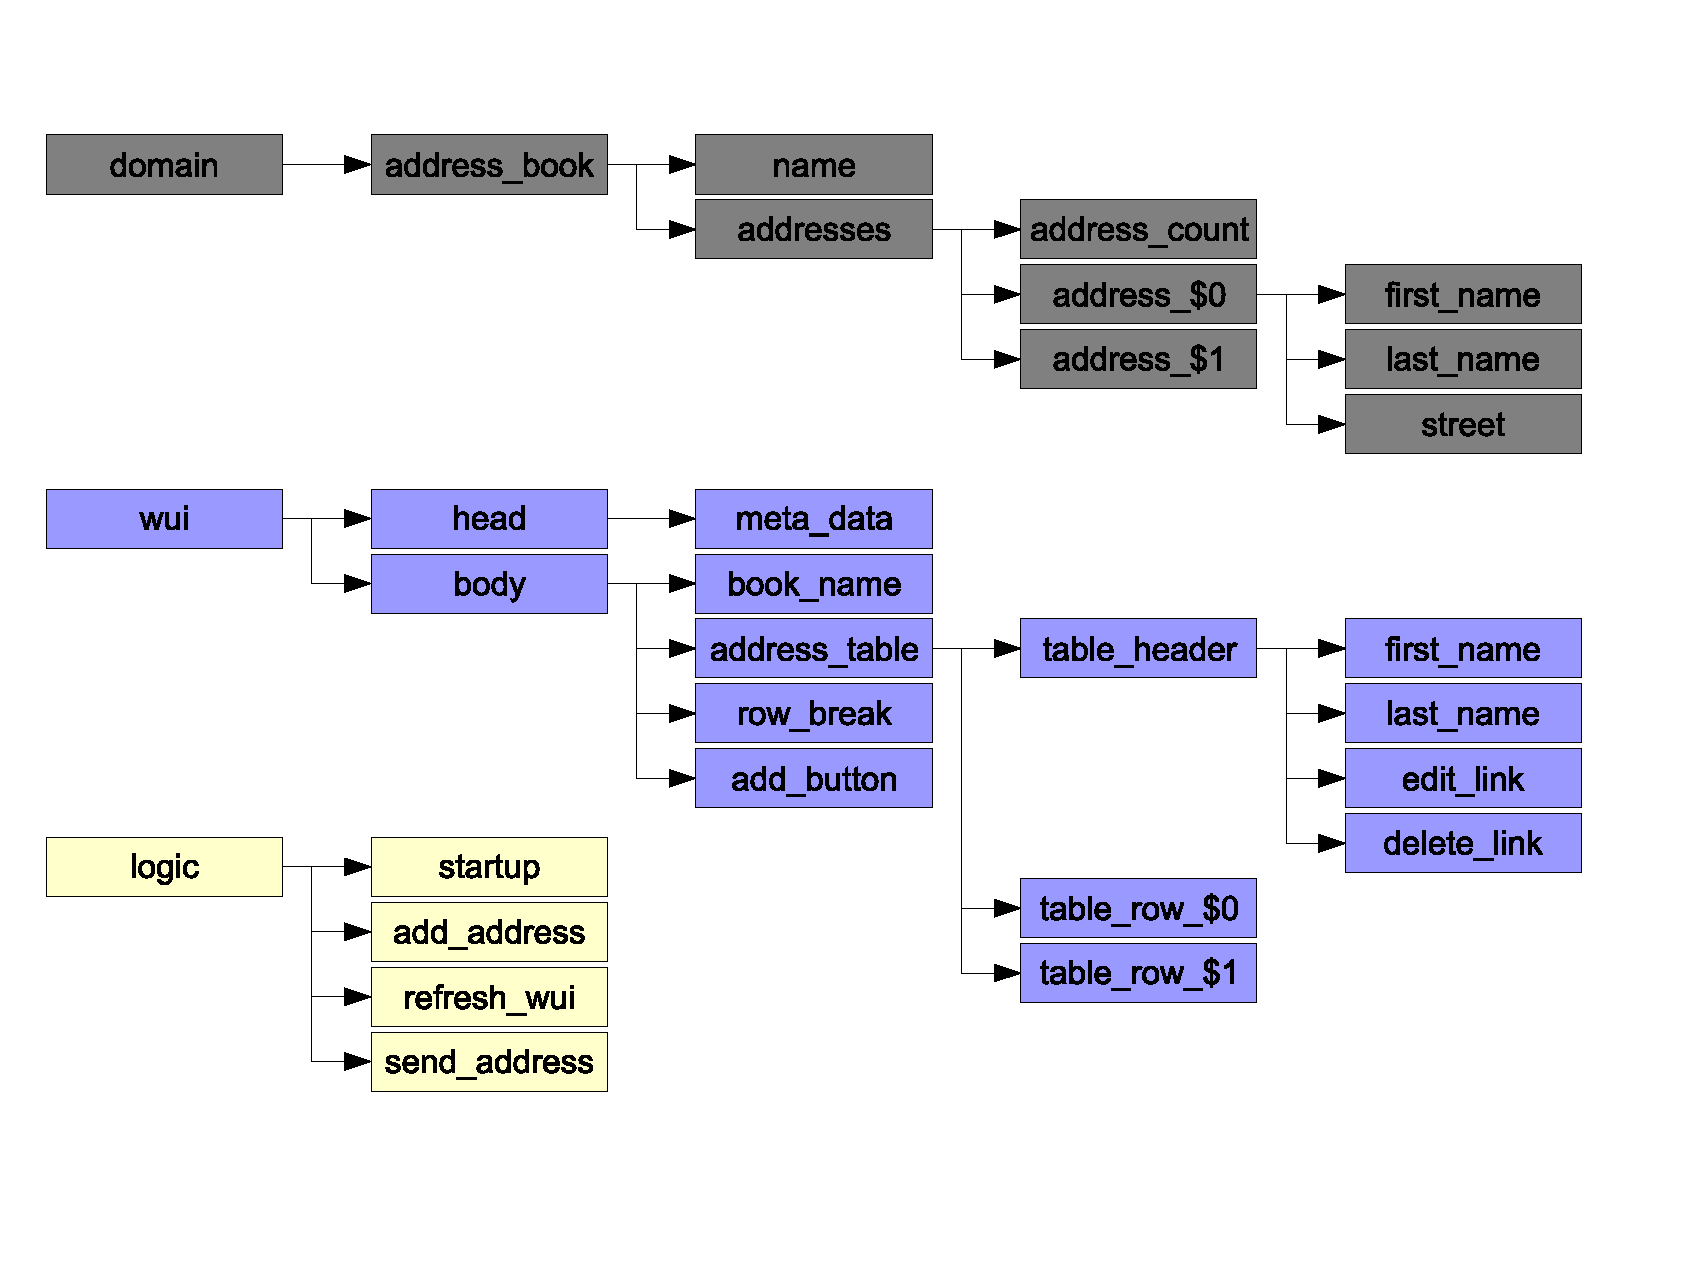
\includegraphics[scale=0.2]{vector/radesign.eps}
        \caption{ResAdmin Knowledge Models}
        \label{radesign_figure}
    \end{center}
\end{figure}

Due to the tremendous complexity of an \emph{Electronic Health Record} (EHR),
only a very small part of its data could be considered for the application
prototype. Administrative data like a person's name or address are standard
information found in all EHRs. A corresponding module named \emph{ResAdmin}
\cite{holzmueller2005} was therefore elected to be realised first. Its models
belong to three categories: \emph{Domain}, \emph{Web User Interface} (WUI) and
\emph{Logic} (figure \ref{radesign_figure}).

The addresses contained in the \emph{domain} branch of the knowledge tree are
manipulated across \emph{Hyper Text Markup Language} (HTML) \emph{User Interface}
(UI) models belonging to the \emph{web} branch of that same tree. An example
structure of a knowledge tree was shown in figure \ref{mvctree_figure}. Every
action model that a user can trigger through the WUI exists as part of the
\emph{logic} branch of the knowledge tree.

Independently of what kind of knowledge model (state or logic) was created,
ontological principles were strictly followed. Most importantly, relations
within a hierarchical model were always \emph{unidirectional}, that is from a
\emph{Whole-} to its \emph{Part} models, but never the other way around.
Additionally, however, logic models may reference and access runtime state
models.

Some of the logic models represent \emph{Translators} (compare section
\ref{communication_model_heading}). They extract address information
residing in the domain- and copy them to the web model, which is afterwards
sent to the human user as communication partner. This principle holds true for
the communication between application systems, only that then other than web
models are used as communication format. The vision to make all communication
channels really \emph{transparent} and easy to handle for the user now seems to
be coming true.
